\chapter{Two Applications of Persistent Homology}
Since our purpose with thesis is not only to give an introduction to persistent homology in terms of theory, but also display how it can be used with actual real-world data, we have investigated two different situations where the theory we have expanded upon so far serve as our main tool for data analysis.

In the first case we quantify differences in morphology between different-sized individuals of the bumblebee \textit{Bombus terrestris} by computing the persistent homology of 3D volumes of their corneas. To our knowledge this is the first use of persistent homology in data pertaining to insects, although in \cite{moon2019, delgadofriedrichs2014} materials and in \cite{gutierrez2012, gutierrez2014} reconstructions of 3D volumes are investigated with approaches that are similar in spirit.

In the second case we try to understand the network structure of the striatum, a part of the basal ganglia in the brain. Due to the sheer computational power needed to compute persistent homology for this data our analysis is more of a holistic summary of the resulting simplicial structure rather than focusing solely on persistent homology. Our approach is largely inspired by \cite{reimann}, in which a similiar analysis is done but for a different part of the brain.

\section{Corneas of Bombus terrestris}
It has been found that the size of individuals of the species \textit{Bombus terrestris} affects aspects of their visual capabilities \cite{emily}. By applying persistent homology we can investigate whether this difference in size also translates to a difference in persistent homology, and so by proxy a difference in topology. If so, this could serve to strengthen the hypothesis that larger individuals have superior, or at the very least different, visual capabilities than smaller individuals. Persistent homology is a good candidate for this purpose as metrics on persistence diagrams are indifferent to differences in scale but rather measures differences in shape.
\subsection{Data}
The data consists of binary 3-dimensional volumes (see Figure \ref{corneas} for renderings of some of the samples) of the corneas acquired by micro-CT scans of the samples described in Table \ref{bees}. The main focus of the analysis will be on samples from the bumblebee \textit{Bombus terrestris}, but in total there are 20 samples belonging to 8 different species of insects. The additional samples from other species will be used to verify our topological findings.
\begin{figure}[h]
  \centering
  \begin{subfigure}{.3 \linewidth}
  \centering
  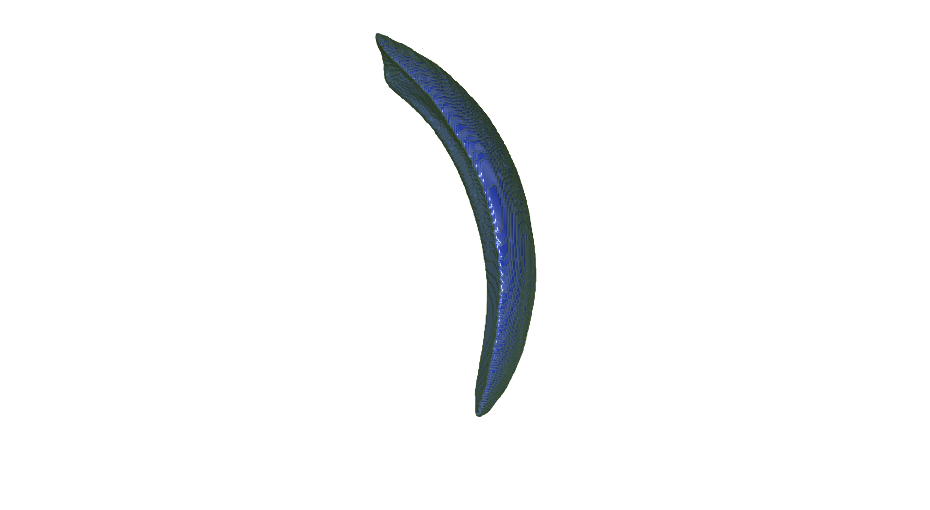
\includegraphics[scale=0.2]{ta60204_cornea.png}
  \caption{TA\_60204}
  \end{subfigure}%
  \begin{subfigure}{.3 \linewidth}
  \centering
  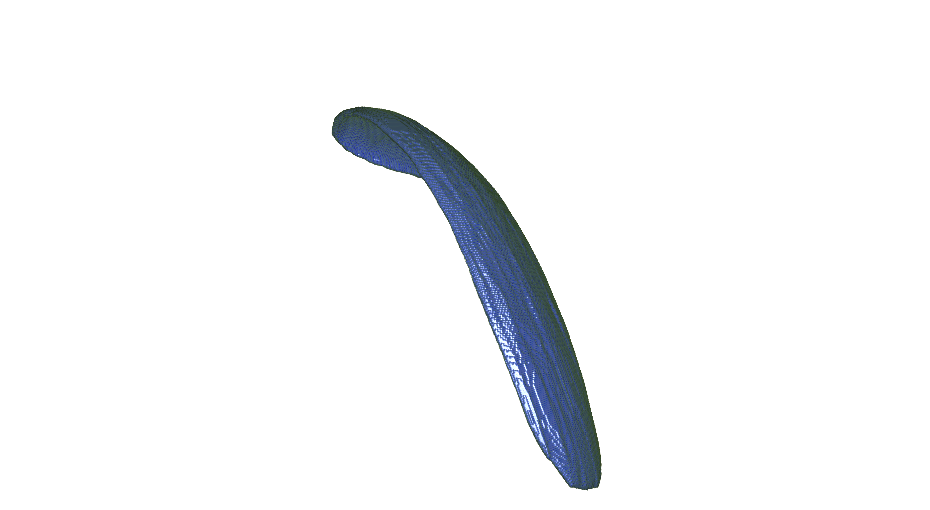
\includegraphics[scale=0.2]{mq60209_cornea.png}
  \caption{MQ\_60209}
  \end{subfigure}%
  \begin{subfigure}{.3 \linewidth}
  \centering
  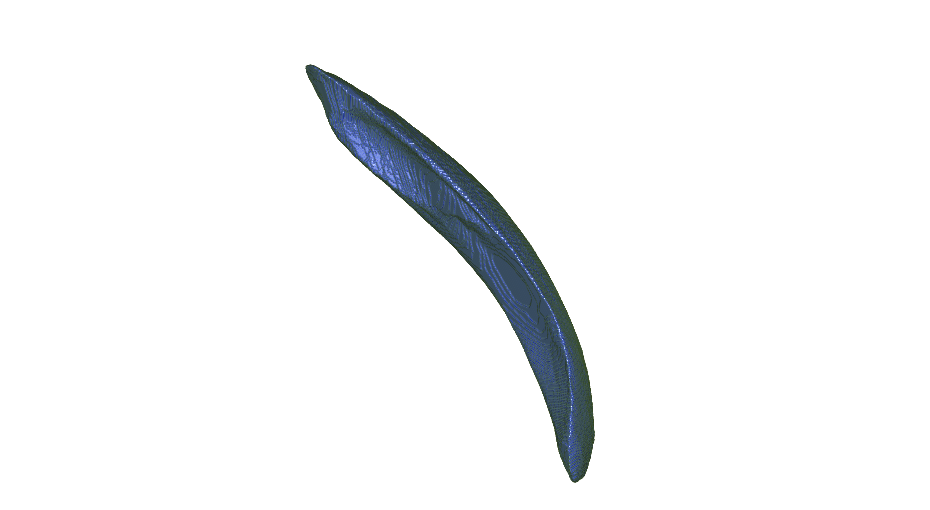
\includegraphics[scale=0.2]{bt77970_cornea.png}
  \caption{BT\_77970}
  \end{subfigure}
  \caption{\label{corneas} Example renderings of cornea volumes.}
\end{figure}
\begin{table}[htb]
\begin{center}
\begin{tabular}{ | c | c | c | }
\hline
  ID & ITW & Species \\
\hline
AM\_60185 & 2.90 & Apis mellifera \\
AM\_60186 & 2.95 & Apis mellifera \\
BT\_77967 & 5.42 & Bombus terrestris \\
BT\_77970 & 4.00 & Bombus terrestris \\
BT\_77971 & 4.02 & Bombus terrestris \\
BT\_77973 & 1.97 & Bombus terrestris \\
BT\_77974 & 2.97 & Bombus terrestris \\
BT\_77976 & 5.47 & Bombus terrestris \\
MB\_60160 & 3.25 & Melipona bicolor \\
MB\_60161 & 3.25 & Melipona bicolor \\
MQ\_60208 & 3.64 & Melipona quadrifasciata \\
MQ\_60209 & 3.64 & Melipona quadrifasciate \\
PR\_60164 & 1.49 & Plebia remota \\
PR\_60206 & 1.49 & Plebia remota \\
TA\_60204 & 1.17 & Tetragonista angustula \\
TA\_78016 & 1.17 & Tetragonista angustula \\
TC\_60166 & 1.94 & Tetragona clavipes \\
TC\_60167 & 1.94 & Tetragona clavipes \\
TS\_60163 & 2.10 & Trigona spinipes \\
TS\_60203 & 2.10 & Trigona spinipes \\
  \hline
\end{tabular}
\caption{Table over the data samples used in the analysis. The ID column gives a unique ID to each sample and the ITW column gives the intertegular width of each sample.}
\label{bees}
\end{center}
\end{table}
\subsection{Methodology}
Since our samples consist of binary 3-dimensional volumes each voxel\footnote{A voxel is the 3-dimensional equivalent of a pixel.} can be considered as cube in a 3-dimensional grid, where a value of $1$ indicates the presence of a cube and a value of $0$ indicates the absence of one. We can exploit this inherent structure in the data and instead of considering simplicial complexes as described in Chapter 2, we can instead impose the structure of a \textit{cubical complex} on the data samples.

\subsubsection{Cubical complexes}
We follow \cite{kaczynski2004} in defining the cubical complex.
\begin{definition}
An elementary interval is a unit interval $[k,k+1]$ or a degenerate interval $[k,k]$ for $k \in \mathbb{N}$.
\end{definition}

\begin{definition}
In an $n$-dimensional space a cube is the cartesian product of $n$ elementary intervals. The dimension of the cube is exactly the number of intervals in the product which are not degenerate.
\end{definition}
Hence, analoguous to simplices a 0-cube is a vertex, a 1-cube is an edge, a 2-cube is a square and a 3-cube is an actual cube in the geometric sense.

From here on the same construction as in simplicial homology holds \footnote{For computational reasons we can also consider the dual cubical complex where we let voxels be the vertices. See \cite{dualcomplex} for a thorough explanation of this.}. We can in the entirely same way as for simplicial homology define a cubical complex and homology on cubical chain complexes.

\begin{example}
  Just like in a simplicial complex the hole highlighted in green in Figure \ref{cubecomplex} is indeed a non-trivial generator of $H_{1}$.
  \begin{figure}[htb]
    \centering
    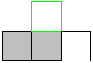
\includegraphics[scale=2]{cubecomplex.pdf}
    \caption{\label{cubecomplex} A cubical complex consisting of two 2-cubes, a 2-cube without the interor and two 1-cubes. }
  \end{figure}
\end{example}

We also need to impose a metric structure on the space given by each sample. Computing the persistent homology of a binary volume will just lead to all cubes in the complex appearing at a threshold of $1$. Instead, we consider the Euclidean Distance Transform (EDT) as a way of imposing a metric structure on the binary volume.

\begin{definition}
  Given a subset $Y \subset \mathbb{R}^{n}$ we define
   \[EDT(x) = \inf_{y \in \partial Y} ||x - y||_2\]
   where $\partial Y$ is the boundary of $Y$.
\end{definition}
So for a given binary volume we embed it in $\mathbb{R}^{n}$ and apply the Euclidean distance transform to get a distance metric between voxels.


\begin{example}
  To calculate the EDT of the binary image in Figre \ref{edt} we simply calculate the difference vector from a cell of value $1$ to the closest cell with value $0$. For example, to get $\sqrt 5$ in the top left corner we need to walk one step in to the left and two steps upwards which translates to the vector $(-1,2)$ which has Euclidean norm $\sqrt{1+4}=\sqrt{5}$.
  \begin{figure}[ht]
    \centering
    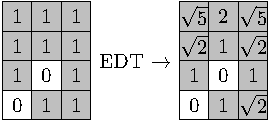
\includegraphics[scale=1.5]{edttransform.pdf}
    \caption{\label{edt} }
  \end{figure}

\end{example}

Our filtration then will describe the structure starting at the boundary of the cornea, the hollow shell surrounding the volume, and then as the threshold increases the cubical complex will include more and more of the denser parts within the volume. An illustration of the thresholding at different values is seen in Figure \ref{thresh}.

\begin{figure}[ht]
  \centering
  \begin{subfigure}{.3 \linewidth}
  \centering
  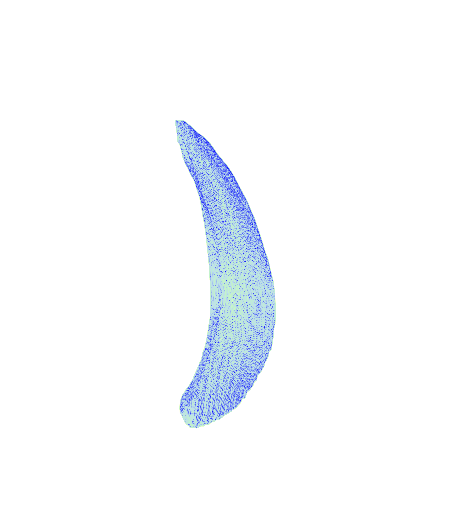
\includegraphics[scale=0.2]{eps2.png}
  \caption{$\epsilon < 2$}
  \end{subfigure}%
  \begin{subfigure}{.3 \linewidth}
  \centering
  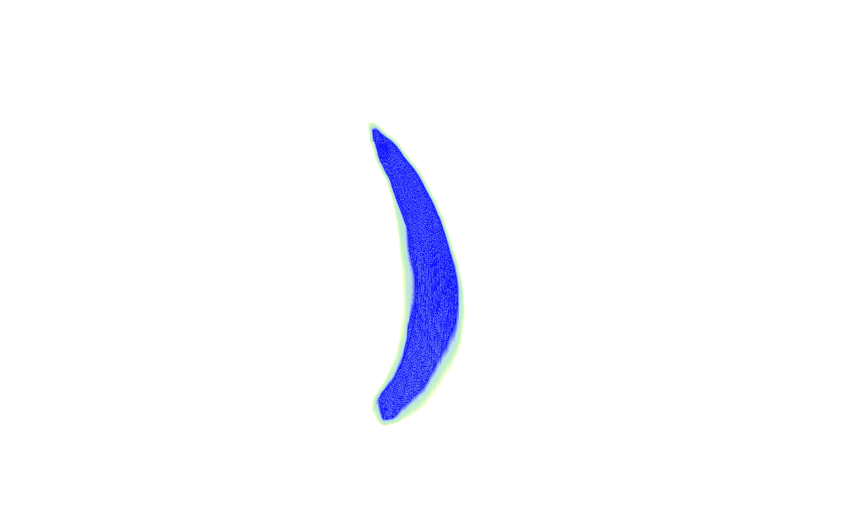
\includegraphics[scale=0.2]{eps10.png}
  \caption{$\epsilon < 10$}
  \end{subfigure}%
  \begin{subfigure}{.3 \linewidth}
  \centering
  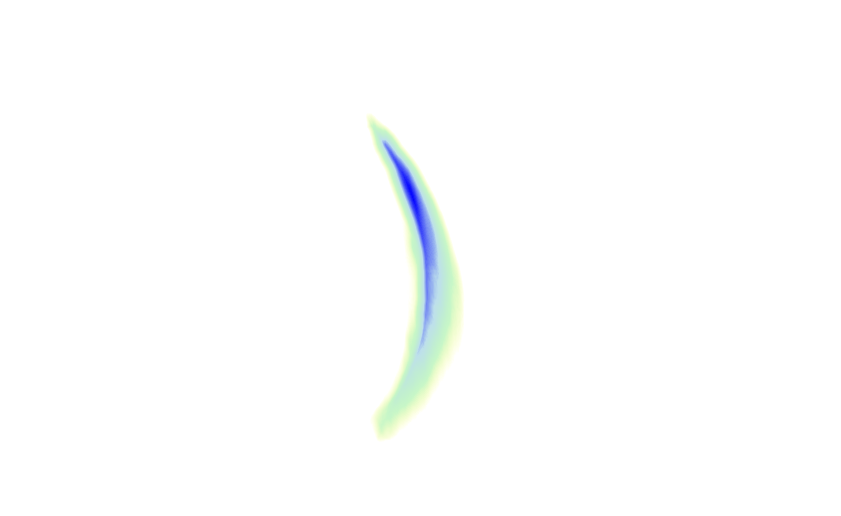
\includegraphics[scale=0.2]{eps100.png}
  \caption{$\epsilon < 100$}
  \end{subfigure}
  \caption{\label{thresh} EDT thresholding of BT\_77976. Cooler colors indicate denser parts of the volume relative to the rest of the volume.}
\end{figure}
The resulting topological summaries we find are barcodes. While these are in themselves interesting, in order to answer whether the size of an individual of the specis \textit{Bombus terrestris} has an impact on the topology of its cornea we compare the samples in a distance matrix, where the metric between pairs is the 1-Wasserstein distance. We choose the Wasserstein distance because it is sensitive to small changes in the persistence diagrams whereas the bottleneck distance only considers the largest differences.

We then analyze this distance matrics using standard tools for data analysis. We are interested in two things:
\begin{enumerate}
  \item Is there a correlation between the size of the bumblebees and their persistent homology?
  \item Can we with persistent homology identify subgroups of bumblebees, and if so are these subgroups related to their size?
\end{enumerate}
Answering these questions will allow us to evaluate whether persistent homology provides information which relates to the hypothesis.

(Work in progress, proper definitions for clustering and Mantel)
In order to identify groupings in the samples we use \textit{hierarchical single-linkage clustering}. Each sample starts out in its own cluster. We then cluster that sample with the sample to which, in terms of persistent homology, it has the lowest distance. We then proceed inductively, and consider the distance from a cluster to another cluster to be the smallest distance among the distances of samples within the two clusters.

To investigate the relationship between between size and topology we additionally compute the distance matrix between the samples' ITWs (intertegular widths) and use the Mantel test to see the correlation between the Wasserstein distance matrix. The Mantel test is a non-parametric test of the correlation between two distance matrices given. The idea is quite simple: we take the two matrices and permute the columns of one of the matrices to compute the probabilities that the values fall within a certain range. If the two matrices are correlated we expect the value to change drastically.
\subsection{Results}
The clusterings on the entire data-set in Figure \ref{wfull1} and Figure \ref{wfull2} reveals that there are two samples of \textit{Bombus terrestris} that are notably different from the other samples of the same species both in their first and second persistent homologies. Coincidentally, these two samples are the samples with the largest ITW in the entire data-set ($5.42$, $5.47$).

We further see that species are mostly grouped together indicating that distances given by 1-Wasserstein between persistent homologies is a capable discriminant when it comes to species. However, there are some oddities such as \textit{Melipona bicolor} and \textit{Melipona quadrifascisata} not being clustered by species.

If we look more closely at \textit{Bombus terrestris} in Figure \ref{wbt1} and Figure \ref{wbt2} we see that persistent homology in both first and second dimension leads to clusterings where the two large samples are considered in a cluster for themselves. However, $H_{2}$ from $H_{1}$ leads to a slightly different clustering where BT\_77971 is considered different from the remaining smaller bumblebees.

\begin{figure}[ht]
  \centering
  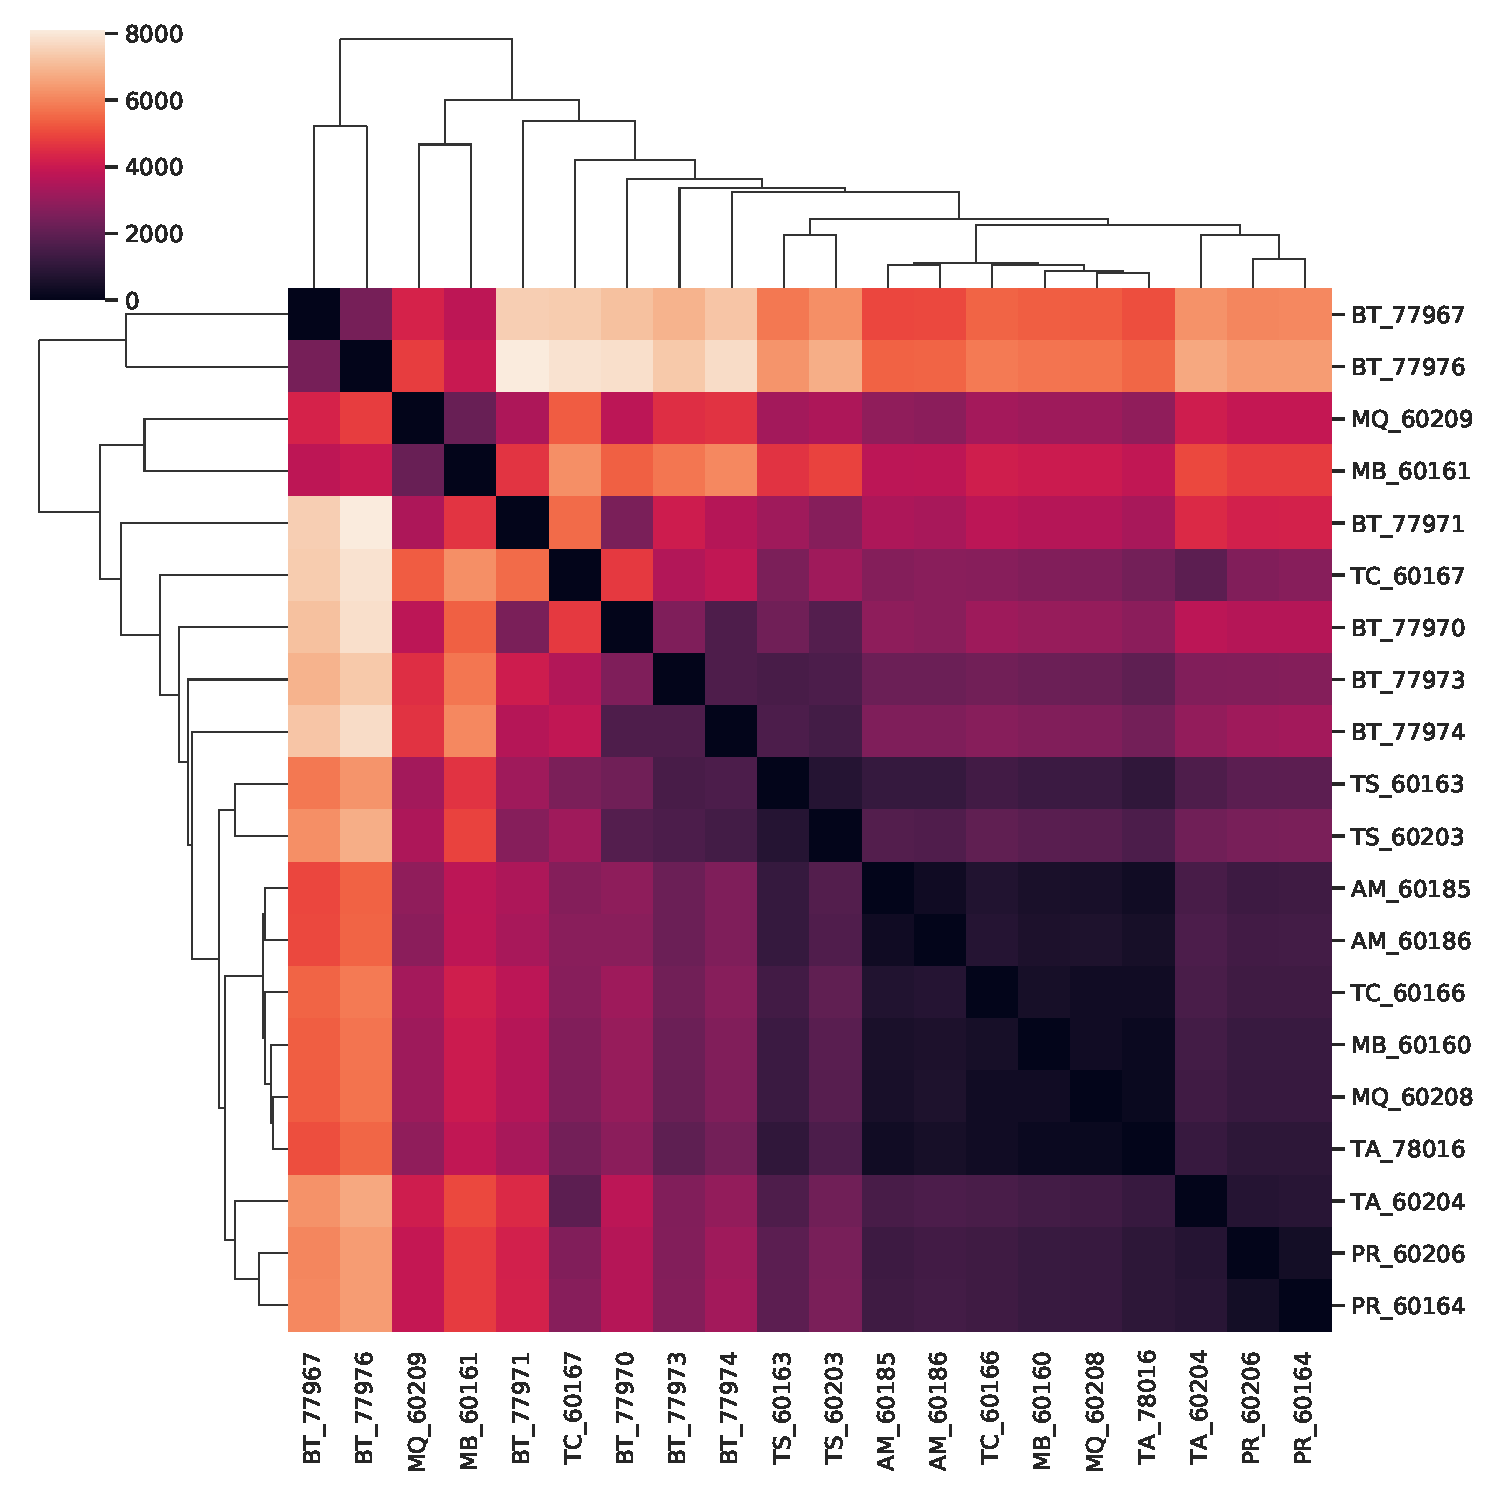
\includegraphics[scale=0.35]{clusters/wasserstein_h1_full.pdf}
  \caption{\label{wfull1} Hierarchical single-link clustering of the 1-Wasserstein distance matrix derived from the persistent homologies of the entire data-set in $H_{1}$.}
\end{figure}



\begin{figure}[h]
  \centering
  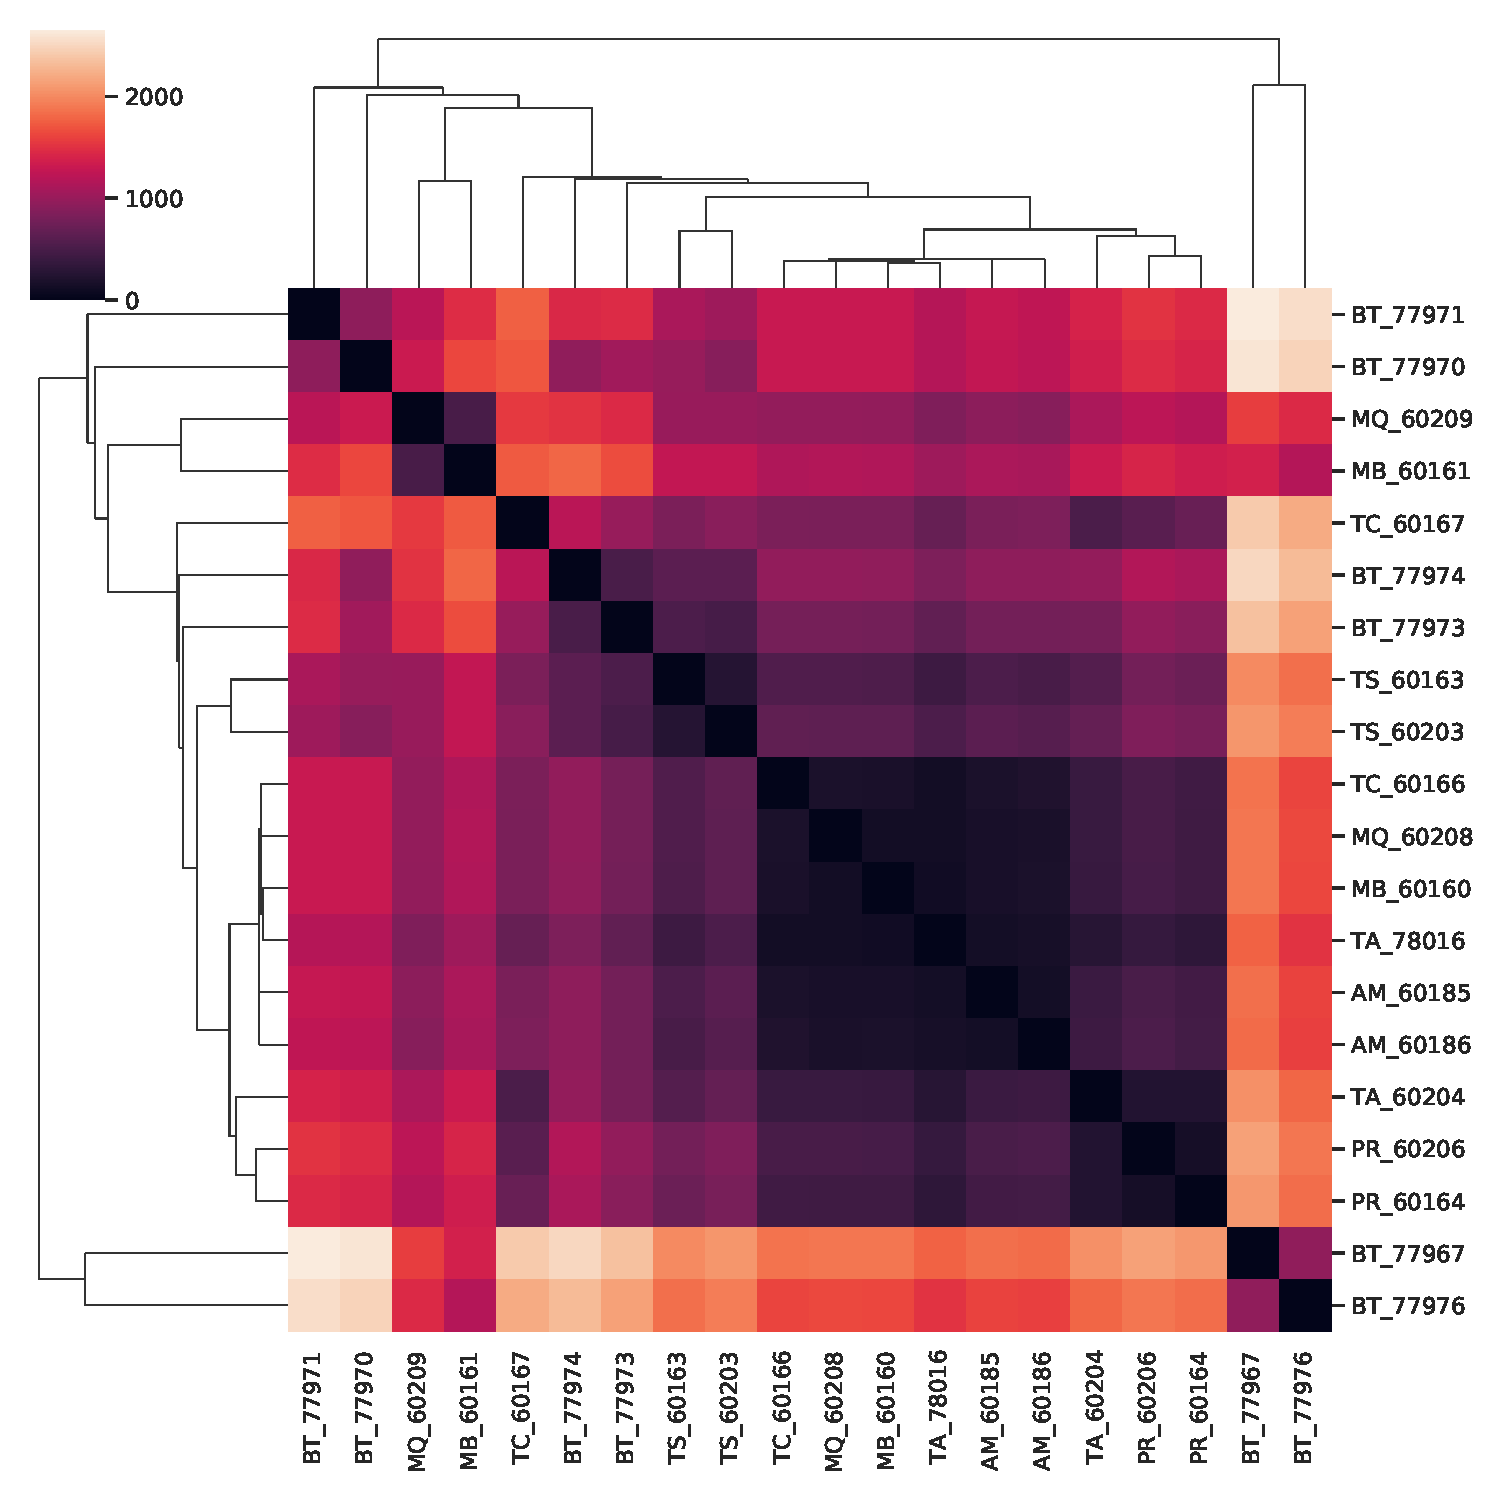
\includegraphics[scale=0.35]{clusters/wasserstein_h2_full.pdf}
  \caption{\label{wfull2} Hierarchical single-link clustering of the 1-Wasserstein distance matrix derived from the persistent homologies of the entire data-set in $H_{2}$.}
\end{figure}

\begin{figure}[h]
  \centering
  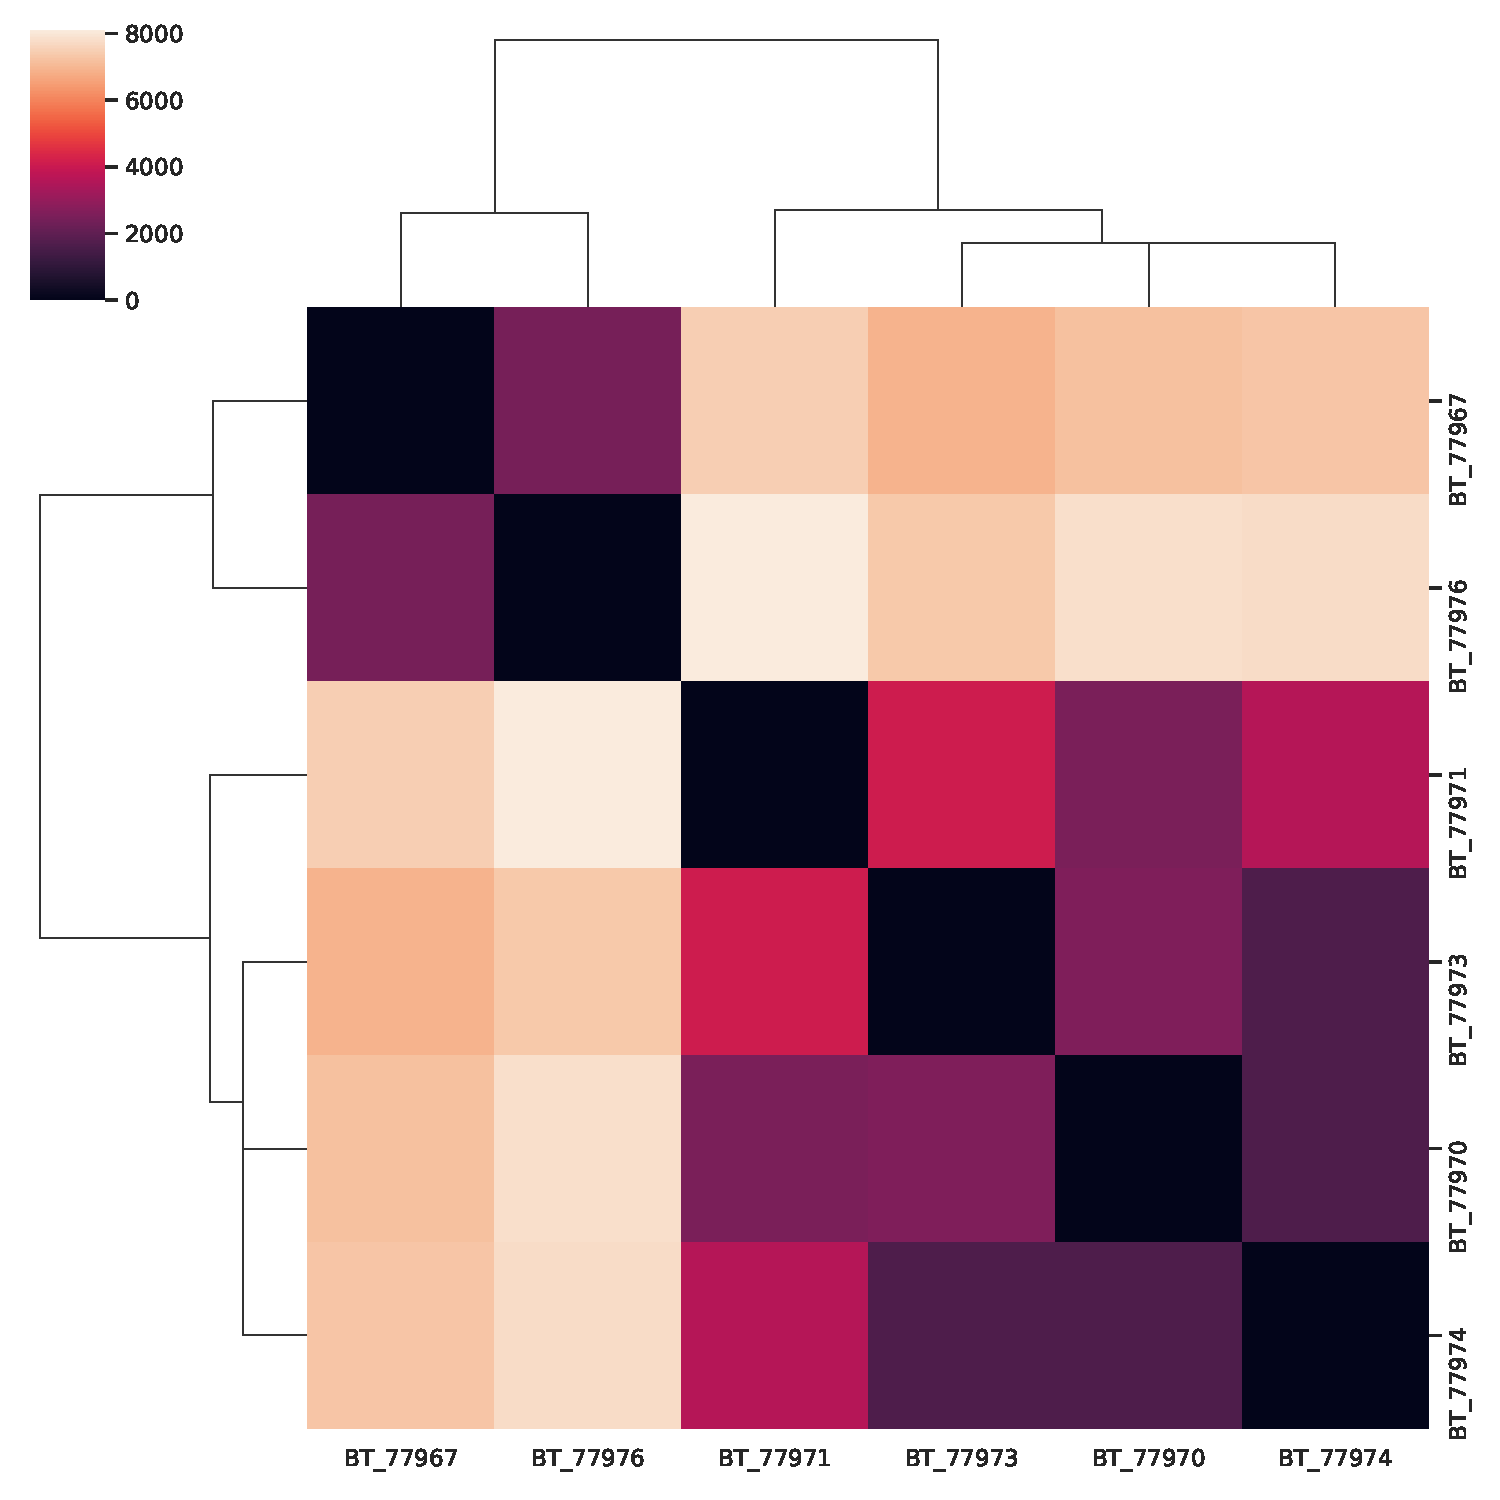
\includegraphics[scale=0.35]{clusters/wasserstein_h1_bt.pdf}
  \caption{\label{wbt1} Hierarchical single-link clustering of the 1-Wasserstein distance matrix derived from the persistent homologies of samples from the species \textit{Bombus terrestris} in $H_{1}$. }
\end{figure}

\begin{figure}[]
  \centering
  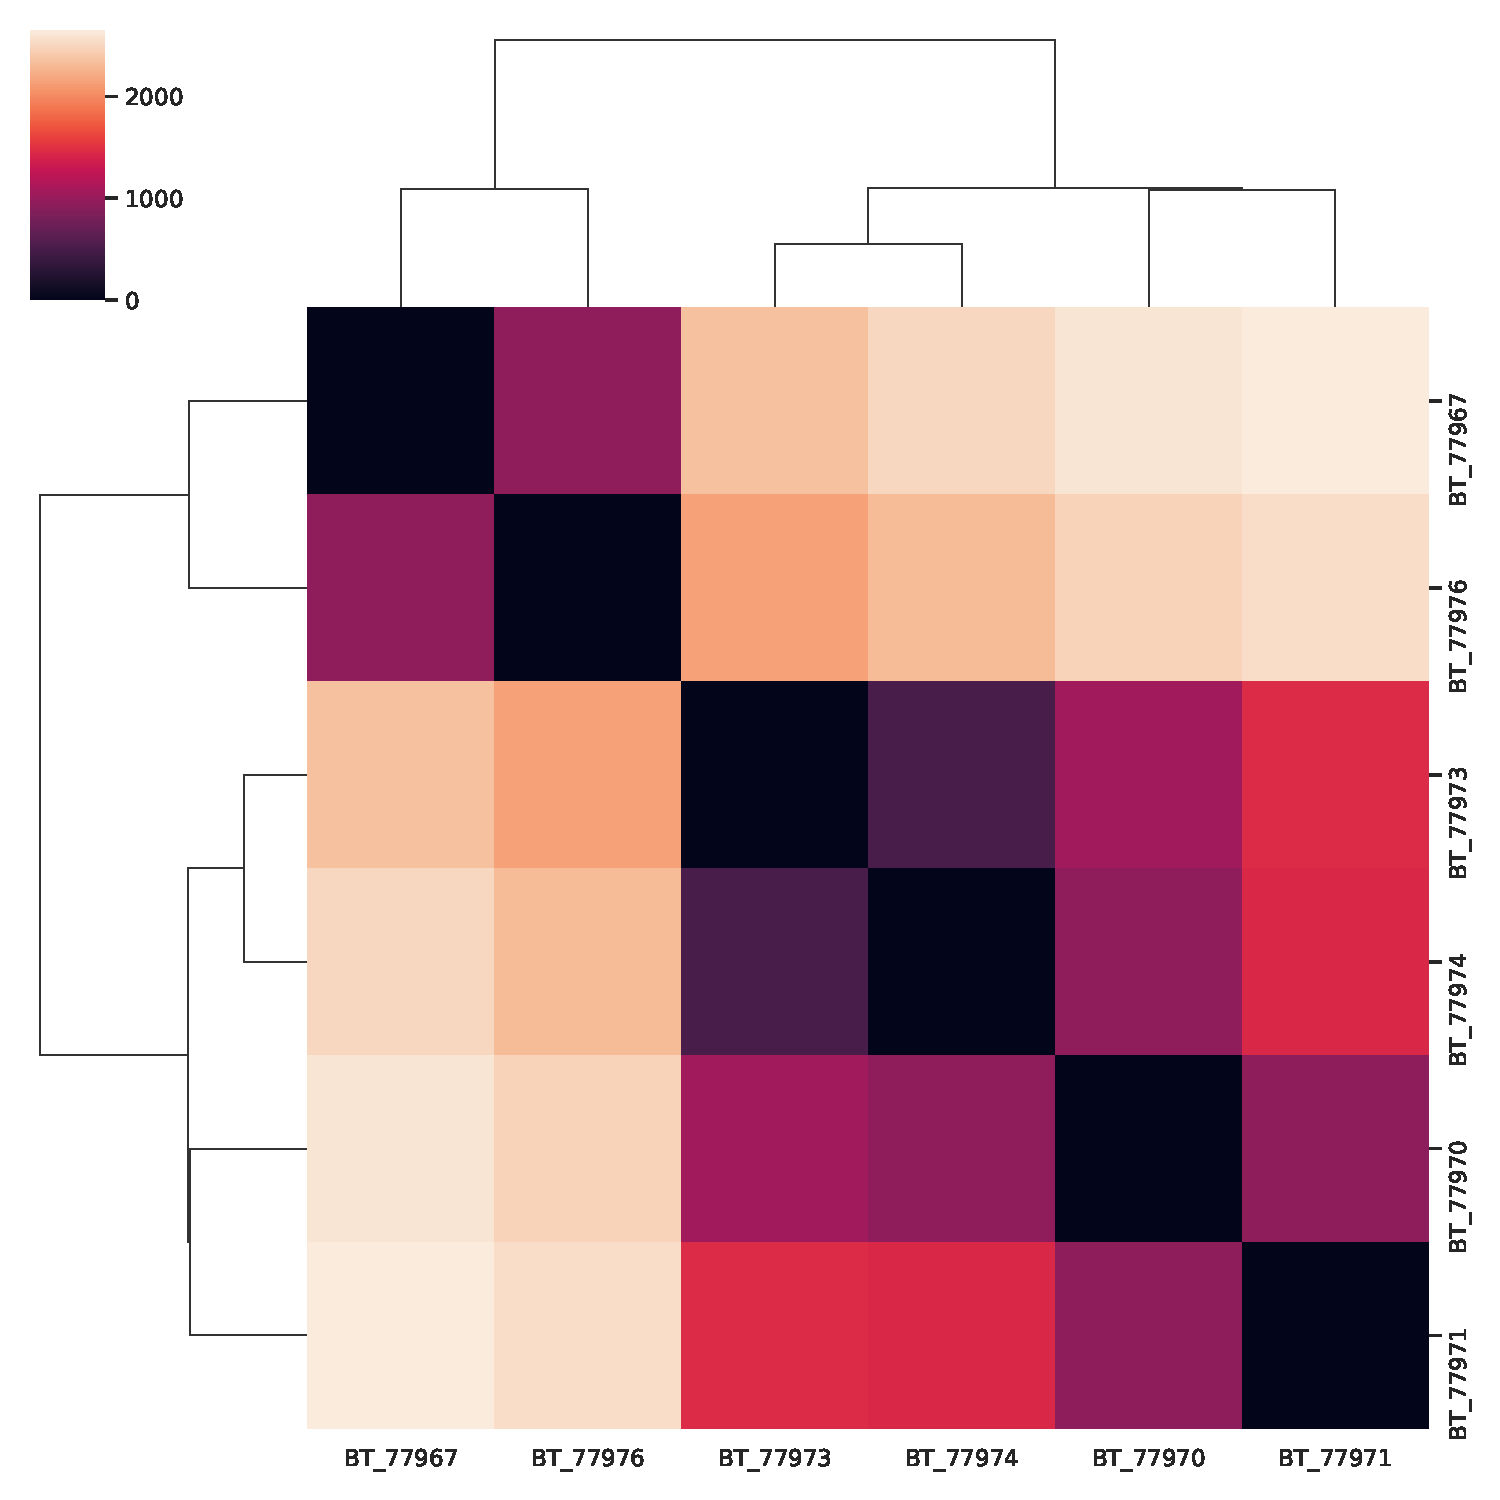
\includegraphics[scale=0.35]{clusters/wasserstein_h2_bt.pdf}
  \caption{\label{wbt2} Hierarchical single-link clustering of the 1-Wasserstein distance matrix derived from the persistent homologies of samples from the species \textit{Bombus terrestris} in $H_{2}$. }
\end{figure}

Finally, we compute the Mantel test and see a non-trivial correlation coefficient for the samples from the species \textit{Bombus terrestris} in Table \ref{mantelc} for the 1-Wasserstein distance in all dimensions. For the significant results we see that we have roughly the same correlation coefficient (0.57) in dimensions 1 and 2 and a weaker one (0.26) in dimension 0.

Notably, none of the bottleneck distances produce any significant results. Perhaps this is not too surprising as the bottleneck distance only provides information about the largest distance in the matching between persistence diagrams. This works well for simple topological shapes, but perhaps too much geometric information is lost about the intermediate stages of the persistent homology filtrations.

\begin{table}[h]
\begin{center}
\begin{tabular}{ | c | c | c | c | }
\hline
  Dimension & Metric & Correlation & P-value \\
  \hline
  0 & Bottleneck & 0.014 & 0.9096 \\
  0 & 1-Wasserstein & 0.26 &  \textbf{0.013} \\
  1 & Bottleneck & -0.11 & 0.4304 \\
  1 & 1-Wasserstein & 0.57 & \textbf{0.0004} \\
  2 & Bottleneck & -0.12 & 0.3415 \\
  2 & 1-Wasserstein & 0.57 & \textbf{0.0003} \\
\hline
\end{tabular}
\end{center}
\caption{\label{mantelc} Table displaying the statistics computed in the Mantel test of the pairwise distances in different dimensions of persistent homology and the ITW for the species \textit{Bombus terrestris}.}
\end{table}
While the purpose of this analysis is mostly a showcase of persistent homology in the wild, these results  do support to the idea that different sized \textit{Bombus terrestris} do not only have larger eyes, but also that they are topologically different. Our clustering results group the larger individuals together and we find a moderate  correlation between the higher order persistent homologies of the samples and their intertegular widths.
\clearpage
\section{Brain network (work in progress)}
Intro. Lorem ipsum.

\subsection{Data}
In this case analysis our main object of study will be two synthetic networks generated based on the striatum.
One network consists of 50 001 vertices and the other network of 999 vertices. It has to be said that the smaller network suffers from being too small to give even the most central neurons all the neighbours it should have.

We follow the results of \cite{reimann} in showing the non-random structure in brain networks.

\subsection{Methodology}
The networks we work with are directed graphs, meaning that a connection from $A \to B$ does not imply a connection from $B \to A$.
\begin{definition}
A directed graph $G={V,E}$ consists of an ordered vertex set $V=(v_{0},\dots)$ and an ordered set of edges $E$ whose elements are of the form $(v_{i},v_{j})$ where the edge in the opposite direction $(v_{j},v_{i})$is not necessarily in the set.
\end{definition}
It is not entirely clear how we should define a simplicial complex on a directed graph, but it is of importance that we try to do so. The assymetry in brain networks are important to capture the structure of how the neurons bind together, and should we disregard the fact that the network is directed important qualities of the network might be lost. While the Vietoris-Rips complex is directly definable on an undirected graph there are a number of different ways to go about defining a similar complex on a directed graph (cite digraph clique article). In our case we follow Reimann et al. (cite) and we extend the notion of the Vietoris-Rips complex, which is a special case of a flag complex, to something called a \textit{directed flag complex} which we construct by imposing a certain partial order on the vertices of the directed graph.

\begin{definition}[\cite{luetdigraph}]
  A directed clique is a directed graph $G=(V,E)$ such that every vertex has at least an outgoing or incoming edge to every other vertex in the graph. \end{definition}

Recall that an ordered (abstract) simplicial complex arises from an ordinary simplicial complex where we give a

\begin{definition}[\cite{luetdigraph}]
  Let G=(V,E) be a directed graph. The directed flag complex dFl(G) is defined to be the ordered simplicial complex whose $k$-simplices are all directed cliques with vertices $v_{0},\dots,v_{k}$ such that $\forall i: v_{i} \in V$
  and $\forall i,j: i < j \implies (v_{i}, v_{j}) \in E$. The vertices $v_{0}, v_{k}$ are called the source and the sink of a $k$-simplex.
\end{definition}

It is important to try to understand this construction because it will have meaning when we try to interpret the homology of the resulting networks. In Figure \ref{disimplex} we see what a $3$-simplex looks like in a \textit{directed flag complex}. We then need to think about what a chain of these directed simplices look like. For example, a $2$-chain of directed simplices can be see in Figure \ref{}. Then what is a cycle? It is a cavity built in by these directed simplices. In the $1$-dimensional case it is not very difficult, it will look something like this.

\begin{figure}[ht]
  \centering
  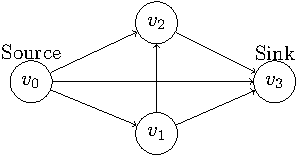
\includegraphics[]{./counts/3simplex.pdf}
  \caption{\label{disimplex} A 3-simplex in a directed flag complex.}
\end{figure}
\subsection{Results}


\begin{figure}[ht]
  \centering
  \begin{subfigure}{.49 \linewidth}
    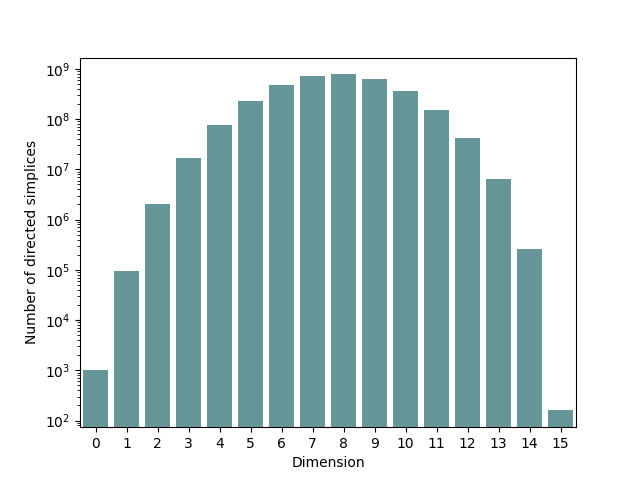
\includegraphics[scale=0.49]{./counts/real1k_count.png}
  \end{subfigure}%
  \begin{subfigure}{.49 \linewidth}
    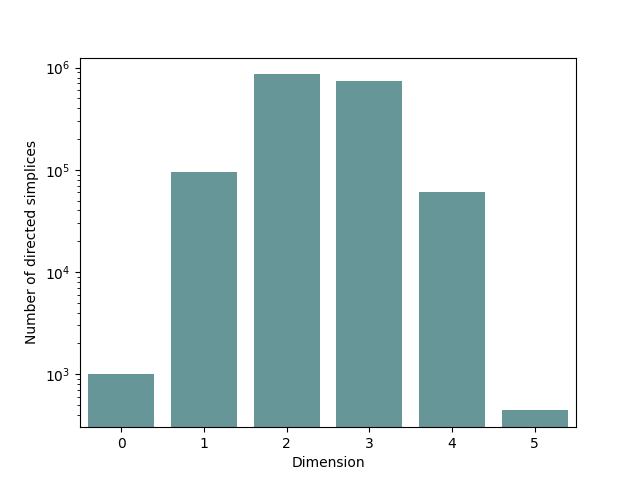
\includegraphics[scale=0.49]{./counts/random1k_count.png}
  \end{subfigure}%
  \caption{\label{count1k}The number of simplices in each dimension for the directed flag complex generated by (a) synthetic network from Snudda, (b) random network generated with the same edge probability creation as the first network, both with 999 vertices.}
\end{figure}

\begin{figure}[ht]
  \centering
  \begin{subfigure}{.49 \linewidth}
    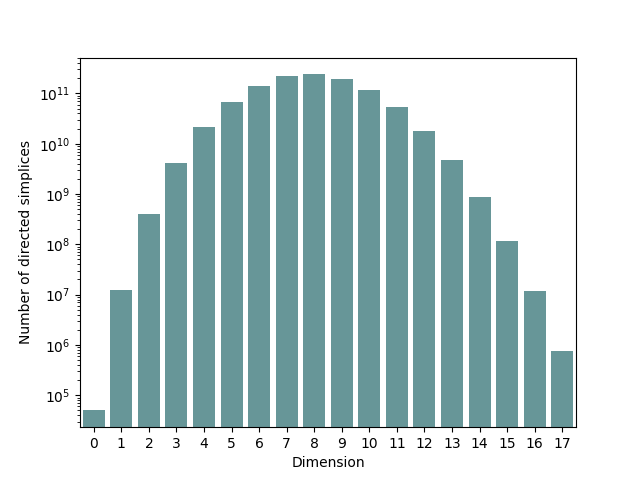
\includegraphics[scale=0.49]{./counts/real50k_count.png}
  \end{subfigure}%
  \begin{subfigure}{.49 \linewidth}
    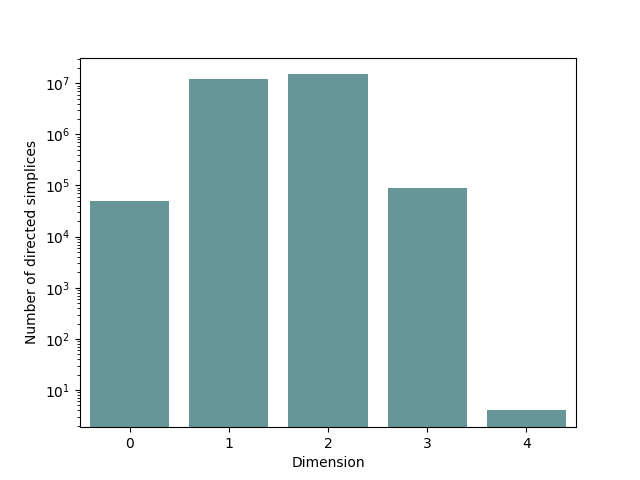
\includegraphics[scale=0.49]{./counts/random50k_count.png}
  \end{subfigure}%
  \caption{\label{count50k}The number of simplices in each dimension for the directed flag complex generated by (a) synthetic network from Snudda, (b) random network generated with the same edge probability creation as the first network, both with 50 001 vertices.}
\end{figure}

In Figures \ref{count1k} and \ref{count50k} we see that the synthetic brain networks have much more higher order structure in terms of high dimensional simplices than a network generated solely based on edge connectivity. For instance, we see in \ref{count50k} the presence of 17-dimensional cells in the synthetic network, which means directed cliques consisting of 18 participating neurons, whereas in the random network we see at most 4-dimensional cell.

In other to further investigate these higher order cells in the synthetic networks we can look at their persistent homology. However, a priori the directed brain network does not have any weights, and so it is not obvious what a filtration $f: V \to \mathbb{R_{+}}$ would look like. So we impose a metric space structure on the directed graph by giving the value of a directed edge between two vertices the Euclidean distance between the two neurons in the simulated model. This means that at low threshold values the filtration will only look at connections made by neurons very close to each other, but as the threshold increases we look at a larger and larger part of the network.

So what is a generator of a homology group in a brain network? It would have to be a $k$-simplex which is not the boundary of a $k+1$-simplex, which translated to the brain network means a clique of neurons that are in themselves an isolated source-sink network and not part of any other network.

Due to computational aspects it is not feasible to compute the persistent homology of the synthetic network with 50 001 vertices, so we restrict ourselves to a subnetwork of the full network consisting only of dSPN neurons as seen in Figure \ref{pers50k}. We also look at a full synthetic network generated with only 999 vertices in Figure \ref{pers1k}.

We see that the formation of higher order $(> 5)$ homology generators mostly happens over small distances, which reaffirms the notion of the brain having a small-world structure.
\begin{figure}[ht]
  \centering
  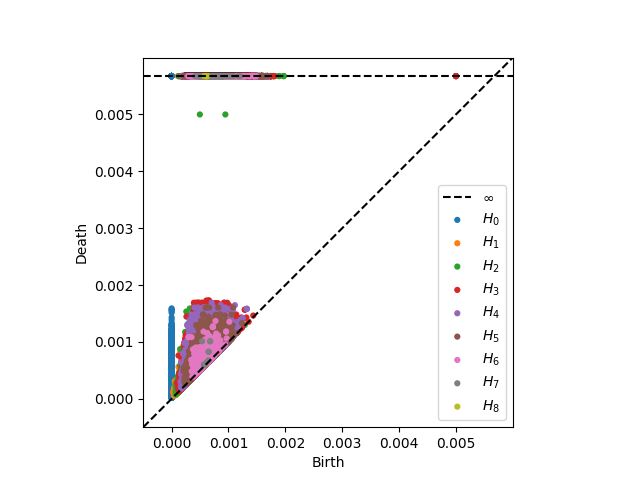
\includegraphics[scale=0.8]{./counts/5kdpsnap10k.png}
  \caption{\label{pers50k} Persistence diagram of the subnetwork of dSPNs extracted from a synthetic network of 50 001 vertices. }
\end{figure}

\begin{figure}[ht]
  \centering
  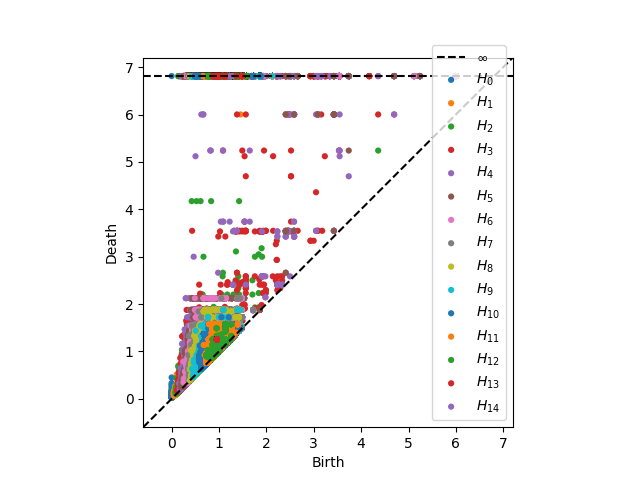
\includegraphics[scale=0.8]{./counts/1kap10000.png}
  \caption{\label{pers1k} Persistence diagram of the entire synthetic network consisting of 999 vertices. (this is scaled 1000 larger than in actual data, generate new diagram)}
\end{figure}
%%% Local Variables:
%%% mode: latex
%%% TeX-master: "thesis.tex"
%%% End:
